\chapter{Detection of cells \statusfirstdraft}
	\label{chap:cell_detection}
	
	\section{Method overview \statusfirstdraft}
	
	In order to track cells across frames we need to first be able to identify the cells within the images. As described in \cref{sec:relatedworkdetection}, there is a broad range of automatic methods for cell detection and segmentation.
	
	The requirements for detecting cells in our application are:
		
	\begin{enumerate}
	\item Accurate detection in sometimes noisy images. The detector should be able to robustly identify cells in datasets that include noise, motion artefacts (induced by the camera and the moving tissue) and variable lens focus. The detector does not need to detect cells that are out of focus, but should reliable detect those are in focus. Out of focus frames are dealt with in the tracking module.
	
	\item There is no need for accurate segmentation. We are primarily interested in the accurate tracking of cells, and analysis of the cells appearance is of secondary interest. For the purpose of tracking, it is sufficient to be able to reliable localize cells, and extract some features that identify these cells.
	
	\item The algorithm should adapt well to different microscopy modalities. The studied datasets are obtained from various organs within the body of mice that have distinct textures. The detector should be able to detect cells in any of these datasets with minimal  manual adjustments.
	\end{enumerate}
	
	Much of the previous work described in \cref{sec:relatedworkdetection} was focused on accurate segmentations of cells. Many of the described methods would return very good segmentations, but they would fail when presented with a very noisy dataset of varying contrast, or need major manual tuning of parameters when presented with a new dataset with a different kind of cells.
	
	For the purpose of our application we have chosen the cell detector presented in \cite{arteta12}, because it conforms to all three requirements. The machine learning method is able to handle noisy datasets, and the model can easily be retrained when a new, previously unseen, type of images needs to be analysed. The method does not focus on accurate segmentation of cells, but on the robust localization. The major drawback of this method was performance. The authors reported run-times of 30 seconds to detect cells on 400-by-400 pixel images on an i7 CPU. This slow performance would make it unusable for tracking large image sequences. However, we were able to optimize the MATLAB code for feature computation so that the detection process takes only a fraction of the original run-time.
	
	The detection process runs in three steps. First, robust candidate regions are extracted from an image. The method uses an efficient MSER region detector \cite{matas04} to find a large number of candidate regions. Second, each of these regions is assigned a value which is produced by a classifier, which indicates the appropriateness score that this this region is a cell. Finally, the non-overlapping subset of these candidate regions with high similarity to the annotated cells in the training data is selected via dynamic programming.
	
	The detector can be trained on a small number of training images, where each cell is  annotated with a single dot. 

	The code used in our method is based on the original code from \cite{arteta12}. Some of our modifications, especially in the feature computations, allow the detector to run significantly faster. Additional work was required to combine the cell detector with the tracking module described in \cref{chap:tracking}.
	
	The remained of this chapter is divided as follows. In \cref{sec:detector_extremal} we describe how the candidate regions are obtained. \Cref{sec:detector_inference} shows the inference procedures that selects the optimal subsets of candidate regions. In \cref{sec:detector_classifier} we formulate the learning method and in we describe the choice of features in \cref{sec:detector_feature}. Finally, in \cref{sec:detector_changes} we briefly outline the main changes that improved the performance of the original algorithm.
	
	\section{Detection of candidate regions \statusfirstdraft}
	\label{sec:detector_extremal}
	
	The first stage of the cell detection process is the extraction of a large number of cell candidate regions. A region is extremal \termmargin{extremal region} if the image intensity everywhere inside of it is highter than the image intensity at its outer boundary. For a grayscale image \textit{I} it is the set of connected components of the thresholded image $\mathcal{I_{>\text{t}}} = \{\mathcal{I} > \text{t}\}$ for some threshold t. In practice we consider only regions that are maximally stable\termmargin{maximally stable extremal region}, as defined in \cite{matas04}, obtained using an efficient maximally stable region detector (MSER).
	
	An important property of extremal regions is \textit{nestedness}, which means that two extremal regions detected on the same image can be either nested or non-overlapping.
	
	The number of obtained candidate regions is high, and an inference step determines which belong to cells.
	
	Extremal regions are invariable to affine transformations of image intensities. They are stable, which means that their support is virtually unchanged over a range of thresholds, they can be detected at multiple scales and can be enumerated very efficiently. This makes them ideal for detecting candidates regions that correspond to cells in microscopy imaging. \Cref{fig:mserexamplesoncells} shows an example result of running the MSER detector on a sample set of microscopy cell images.
	
	\begin{figure}[h]
		\centering
		\missingfigure{Examples of MSER detections}
		\caption{Mser detection examples}
		\label{fig:mserexamplesoncells}
	\end{figure}
	
	\section{Inference under the non-overlap constraint \statusfirstdraft}
	\label{sec:detector_inference}
	
	The inference procedure selects a subset of candidate extremal regions that corresponds to cells. Let $V_i$ be a value assigned to each candidate region $R_i$ indicating the appropriateness of the region to correspond to a cell. The inference procedures selects a subset of the non-overlapping candidate regions such that the sum of the values of selected regions is maximized. To make the problem computationally feasible, the regions are organized into tress according to the nestedness property. Each tree represents a set of overlapping extremal regions. The problem can then be formalized as followes. Let $\textbf{y} = \{y_1, y_2, \dots y_N\}$ be binary variable such that $y_i = 1$ if the region $R_i$ is selected. Let $mathcal{Y}$ be the set of non-overlapping regions. The maximization problem can be defined as:
	
	\[
		F(\textbf{y}) = \max_{\textbf{y} \in \mathcal{Y}} \sum_{i=1}^N y_i V_i \text{.}
	\]
	
	Further details on how the exact solution is obtained can be found in \cite{arteta12}.
	
	Although cells in the studied datasets occasionally overlap, detecting only non-overlapping cells is a good balance between manual work required to annotate datasets, training time and accuracy of the detections. The described framework has been expanded to learn to detect partially overlapping regions \cite{arteta13}. However, that model requires a longer training time, and a larger set of manually annotated images to accurately detect blobs of overlapping cells. Finally, the global data association technique used in the cell tracker module should be able to correctly associate cells if the overlap time is short, such as in trajectories that are crossing and then continuing in opposite directions.
	
	
	\section{Learning the classifier \statusfirstdraft}
	\label{sec:detector_classifier}
	
	The value $V_i$ assigned to each region $R_i$ is a classifier score that indicates the similarity of the extremal region to a cell. The classifier is trained using dot-annotated training images $\mathcal{I}^1, \mathcal{I}^2, \mathcal{I}^3, \dots$ as follows. Let $R_1, R_2,\dots,R_{N^j}^j$ indicate the set of $N^j$ candidate regions extracted from the training image $\mathcal{I}^j$. The value $V_i^j$ of each region is computed as the dot product between a feature vector $\textbf{f}_i^j$ computed for each region and a weight vector $w$: $V_i^j = \textbf{f}_i^j \cdot w$.
	
	The learning procedure has to learn the weight vector $w$ so that the inference procedure tends to pick regions with a single annotated cell $n_i^j = 1$. In order to consider the non-overlap constraint of regions a structured SVM \cite{tso04} is used that directly optimizes the performance of the inference on the training set. The loss function that the learning framework tries to optimize counts the number of deviations from the one-to-one correspondence between the annotated dots and the selected regions:
	
	\[
		L(\textbf{y}^j) = \sum_{i=1}^{N^j} y_i^j |n_i^j - 1| + U^j(\textbf{y}^j)\text{,}
	\]
	
	where $n_i^j$ indicates the number of annotated dots in region $R_i^j$ and $U^j(\textbf{y}^j)$ counts the number of annotated dots that do not have a corresponding selected region $R_i^j$. Further details about the convex objective we try to minimize and how it can be optimized using a cutting-plain algorithm can be found in \cite{arteta12}.
		
	\section{Feature selection \statusfirstdraft}
	\label{sec:detector_feature}
	
	The effictiveness of the machine learning method to detect cells depends on the quality of features computed for the regions. Good features have a lot of discriminative power, so that they can effectively distinguish regions corresponding to cells to regions that don't correspond to cells. In order to find the best feature vector we have evaluated the performance of the classifier with several combinations of these features:
	
	\begin{enumerate}
	    \item The area A of the region represented by a 10-dimensional binary vector with the entry $\lceil log A \rceil $ set to 1.
		\item 10-dimensional histogram of intensities within the region.
	    \item The position of the descriptor in the image in terms of x-y coordinates of a centroid fitted to the descriptor.
	    \item Two 6-dimensional histograms of differences in intensities between the region border and a dilation of it for two different dilation radii.
	    \item A shape descriptor represented by a 60-dimensional histogram of the distribution of the boundary of the region on a size-normalized polar coordinate system.
	    \item The orientation of the descriptor after attempting to normalize its orientation.
	    \item The proportion of edge-pixels in the region.
	\end{enumerate}
	
	Each of these features has different discriminative power, and takes some time to compute. The application of the cell detector requires that images are processed within a time limit. For this reason, we have trained and tested the algorithm with all the $2^7 - 1$ possible combinations of these features.
	
	We have also developed a tool that helps select the most appropriate set of features given specific constraints, for example a maximum computation time, minimal precision and recall values, etc. A graph generated by the function is shown in figure \ref{fig:bestFeatureSelector}.
	
	\begin{figure}[h]
		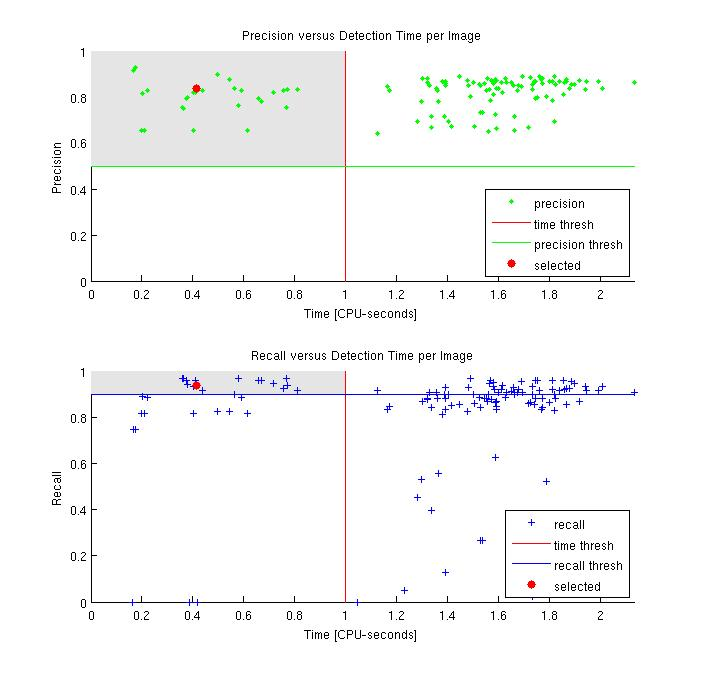
\includegraphics[width=\textwidth]{images/best_features}
		\caption{The plots helps the user to select an appropriate feature set according to the computation time per image, mean precision and recall. This example filters features sets that compute within 1 CPU-second per image (on average), have at least 0.5 precision and 0.9 recall. The feature set corresponding to the red dots contains features 1, 3 and 4. Most importance was given to high precision followed by low computation time and high recall. The selected feature set computes in about 0.4 CPU-seconds per 512-by-512 pixel image with mean precision of 0.836 and mean recall of 0.9363 (as measured on an i7-2600 CPU wish a clock frequency of 3.40 GHz).}
	    \label{fig:bestFeatureSelector}
	\end{figure}
	
	\section{Performance improvements \statusfirstdraft}
	\label{sec:detector_changes}
		The main drawback of the algorithm presented by Arteta \cite{arteta12} is the slow feature computation. The original algorithm took about 30 seconds to detect cells in a 400-by-400 pixel image. Because the aim of this project is tracking cells, we expect to be processing hundreds or thousands of frames of microscopy image sequences. It was important to reduce the detection time as much as possible. The major performance improvements where achieved by addressing three things.
		
		The algorithms computes the features for the classifier on every candidate maximally extremal region. The original method was configured such that thousands of MSERs were computed for each frame. While this provides more robust learning and detection, it was slowing the algorithm down excessively. First, we have first fine-tuned the MSER detector to detect less regions, but still return a large number of features such that the detection rate wasn't penalized.
		
		Second, we have identified the slowest computed features and improved the algorithmic behaviour of the original MATLAB implementation. One such feature is the Contour Points Distribution Histogram. The function was performing many calls to slow built in functions to extract region characteristics. This, and other functions, were rewritten to call these expensive sub-procedures less frequently, without affecting their behaviour.
		
		Third, we noticed that the MATLAB built-in function were performing a lot of parameter checking, to make sure that the input parameters were valid. Many of these parameters were strings, and string manipulations are very slow in MATLAB. Several MATLAB built-in function were rewritten or modified to remove excessive parameter checking, which in several cases represented an overhead of over $30\%$. These parameter checks are welcome when developing the algorithm, but once the algorithm is complete, several of these checks can be safely removed.
		
		It is also worth mentioning that the updated original code for the detector is now stabler and better tested. A few rare bugs have been fixed, after being found when running the detector over large number of datasets.
		
		These optimizations resulted in a significant performance boost. The updated algorithm can perform the same computations in a fraction of the time taken by the original implementation provided by the authors of \cite{arteta12}.
	